\section{Experiments and Results}

\subsection{Main Results}

Table~\ref{tab:main_results} summarizes the key experimental results.
All values are reported on the held-out test set.
Experiments are ordered to reflect the progression of design choices: baseline, preprocessing, attention placement, optimizer, and loss function.

\begin{table*}[ht]
\centering
\caption{Test set results for selected experiments. Best Mean Test AUC is shown in \textbf{bold}. Best Recall and F1 are \underline{underlined}. All threshold-based metrics are computed at 0.5.}
\label{tab:main_results}
\setlength{\tabcolsep}{5pt}
\begin{tabular}{llccccc}
\toprule
\textbf{Exp} & \textbf{Configuration} & \textbf{Best Val AUC} & \textbf{Mean Test AUC} & \textbf{Precision} & \textbf{Recall} & \textbf{F1} \\
\midrule
01 & DenseNet121 + BCE                              & 0.8319 & 0.8352          & 0.4226 & 0.1181          & 0.1700          \\
02 & DenseNet121 + CLAHE + BCE                      & 0.8321 & 0.8339          & 0.4195 & 0.1310          & 0.1843          \\
03b & DenseNet121 + CLAHE + CBAM block34 + BCE       & 0.8320 & 0.8359          & 0.4044 & 0.1050          & 0.1451          \\
07 & DenseNet121 + CBAM block34 + BCE + Adam        & 0.8344 & 0.8361          & 0.4421 & 0.1284          & 0.1790          \\
08 & DenseNet121 + CBAM block34 + BCE + AdamW       & 0.8338 & \textbf{0.8371} & 0.4482 & 0.1395          & 0.1962          \\
09 & DenseNet121 + CBAM block34 + ASL + AdamW       & 0.8323 & 0.8370          & 0.3865 & \underline{0.2385} & \underline{0.2736} \\
10 & DenseNet121 + CBAM block34 + Focal($\gamma{=}2$) + AdamW & 0.8336 & 0.8351 & 0.4391 & 0.1258          & 0.1769          \\
\bottomrule
\end{tabular}
\end{table*}

\textbf{Experiment~08} achieves the highest Mean Test AUC of 0.8371, using CBAM block34 with BCE and AdamW without CLAHE preprocessing.
\textbf{Experiment~09} achieves nearly identical AUC (0.8370, $\Delta = -0.0001$) while substantially improving Recall (+0.0990) and F1 (+0.0774) by replacing BCE with Asymmetric Loss.

\subsection{Overview of All Experiments}

Figure~\ref{fig:all_auc} shows Mean Test AUC across all 14 experimental configurations.
The AUC values are closely clustered in the range 0.824--0.837, indicating that the core DenseNet121 architecture provides a strong and consistent baseline.
Experiment~08 achieves the highest AUC, and the no-CLAHE experiments (07--10) generally outperform the CLAHE-based experiments (02--05b).

\begin{figure}[H]
  \centering
  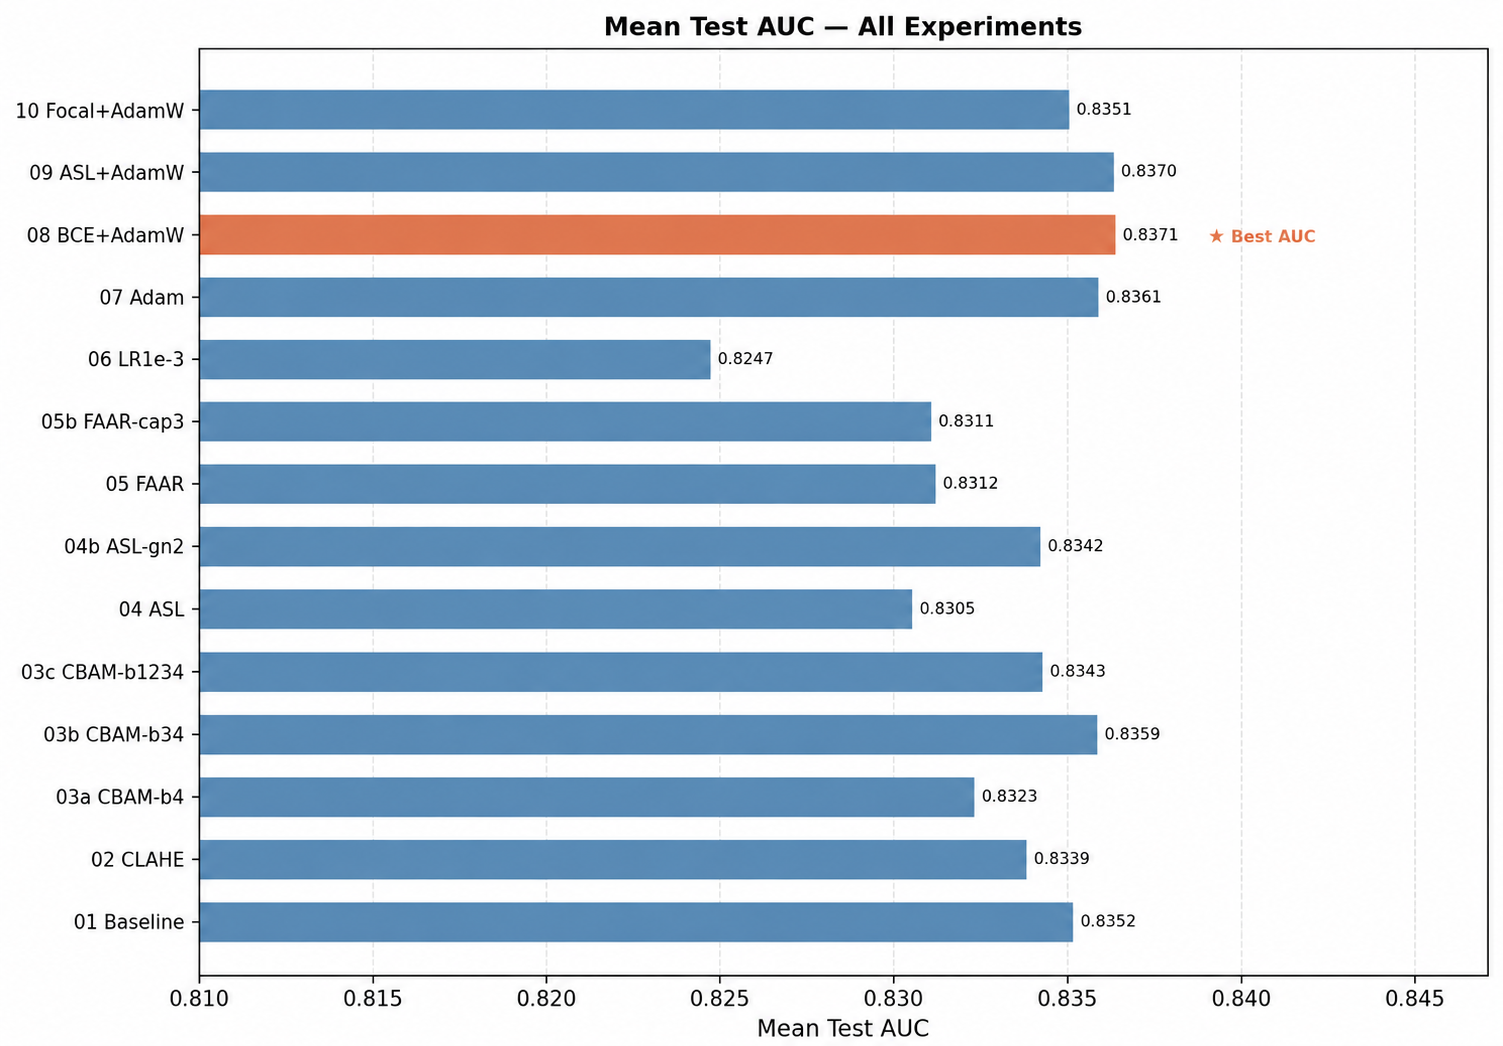
\includegraphics[width=\linewidth]{figures/all_experiments_mean_test_auc.png}
  \caption{Mean Test AUC for all 14 experimental configurations.
    Experiment~08 (highlighted) achieves the highest mean AUC of 0.8371.
    No-CLAHE experiments (07--10) generally outperform CLAHE-based ones.}
  \label{fig:all_auc}
\end{figure}

\subsection{Best Models Comparison}

Figure~\ref{fig:best_compare} directly compares Experiments~08 and~09 across all four reported metrics.
While both models achieve comparable AUC, the ASL model (Exp~09) shows markedly higher Recall and F1, demonstrating the trade-off between precision-oriented and recall-oriented objectives.

\begin{figure}[H]
  \centering
  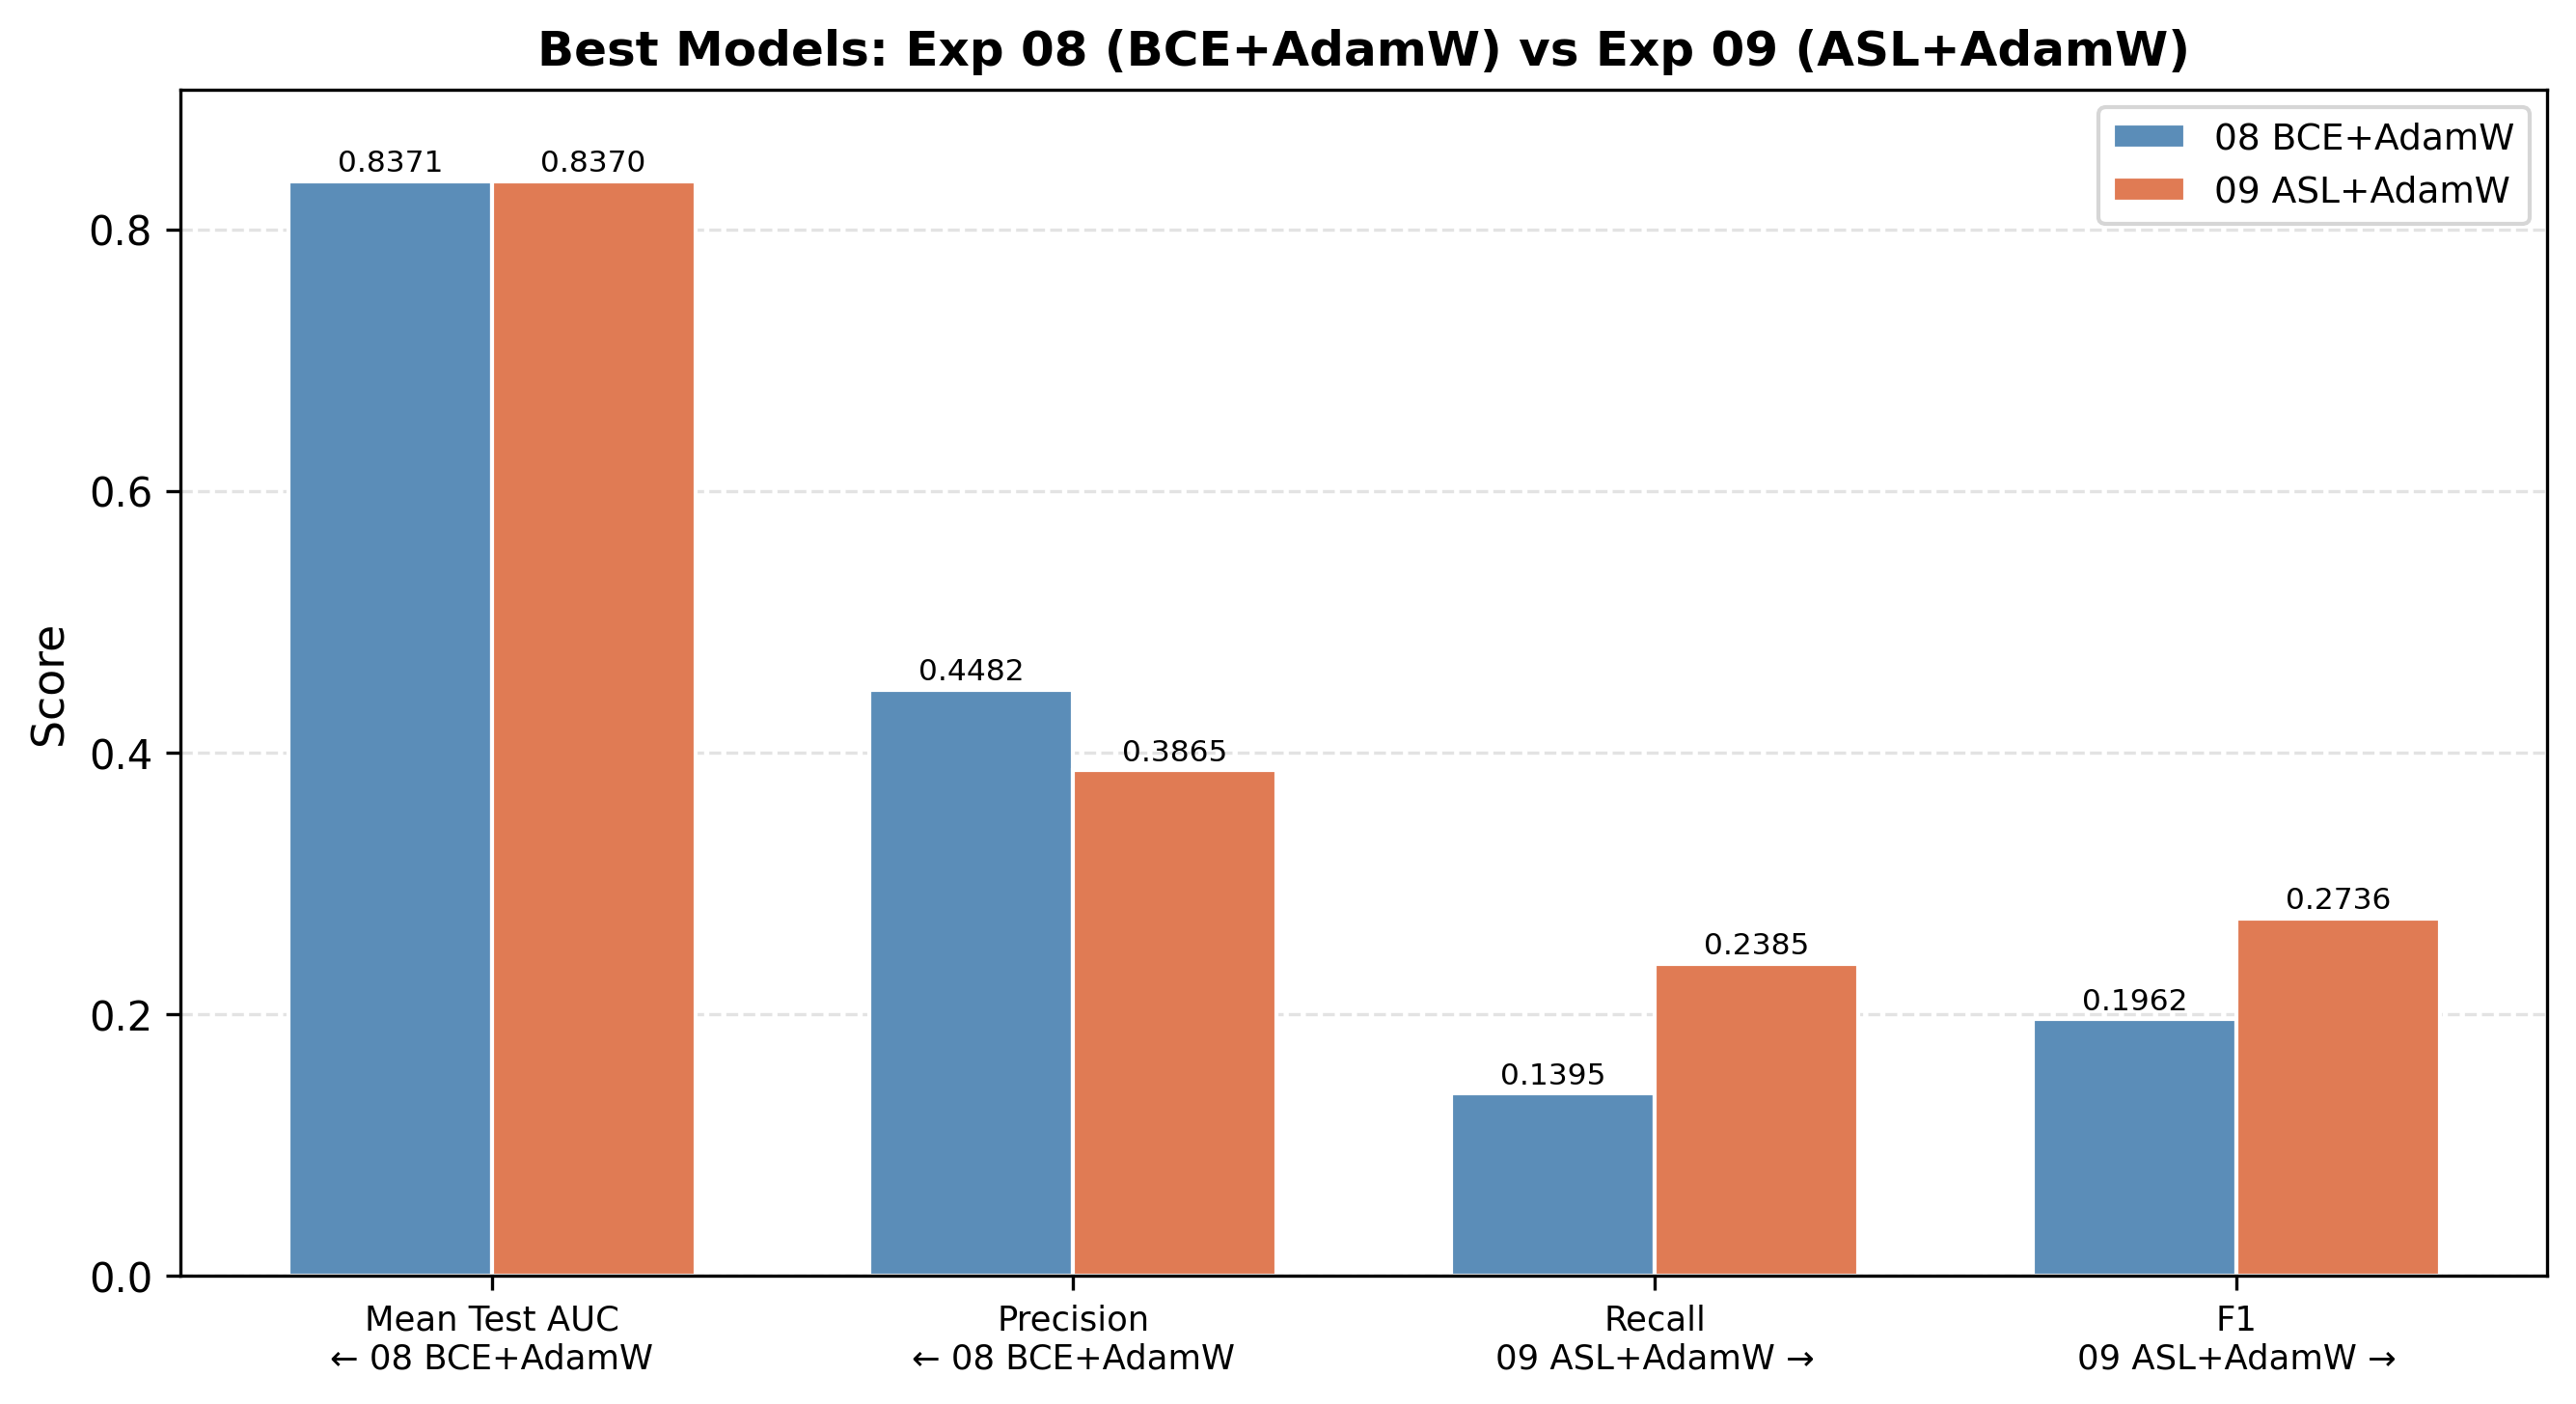
\includegraphics[width=\linewidth]{figures/final_best_models_comparison.png}
  \caption{Metric comparison between Experiment~08 (BCE + AdamW) and Experiment~09
    (ASL + AdamW). AUC values are nearly identical; Exp~09 achieves substantially
    higher Recall and F1 at the cost of lower Precision.}
  \label{fig:best_compare}
\end{figure}

\subsection{Per-Class AUC}

Figure~\ref{fig:perclass} shows per-class AUC for Experiments~08, 09, and~10.
All three models perform well on Hernia (AUC~$\approx$~0.92--0.94), Emphysema ($\approx$~0.92--0.93), Edema ($\approx$~0.90), and Cardiomegaly ($\approx$~0.90).
The most challenging classes are Infiltration ($\approx$~0.72), Pneumonia ($\approx$~0.74), and Nodule ($\approx$~0.75).
These difficult classes tend to have higher prevalence or greater visual overlap with other conditions.

\begin{figure*}[ht]
  \centering
  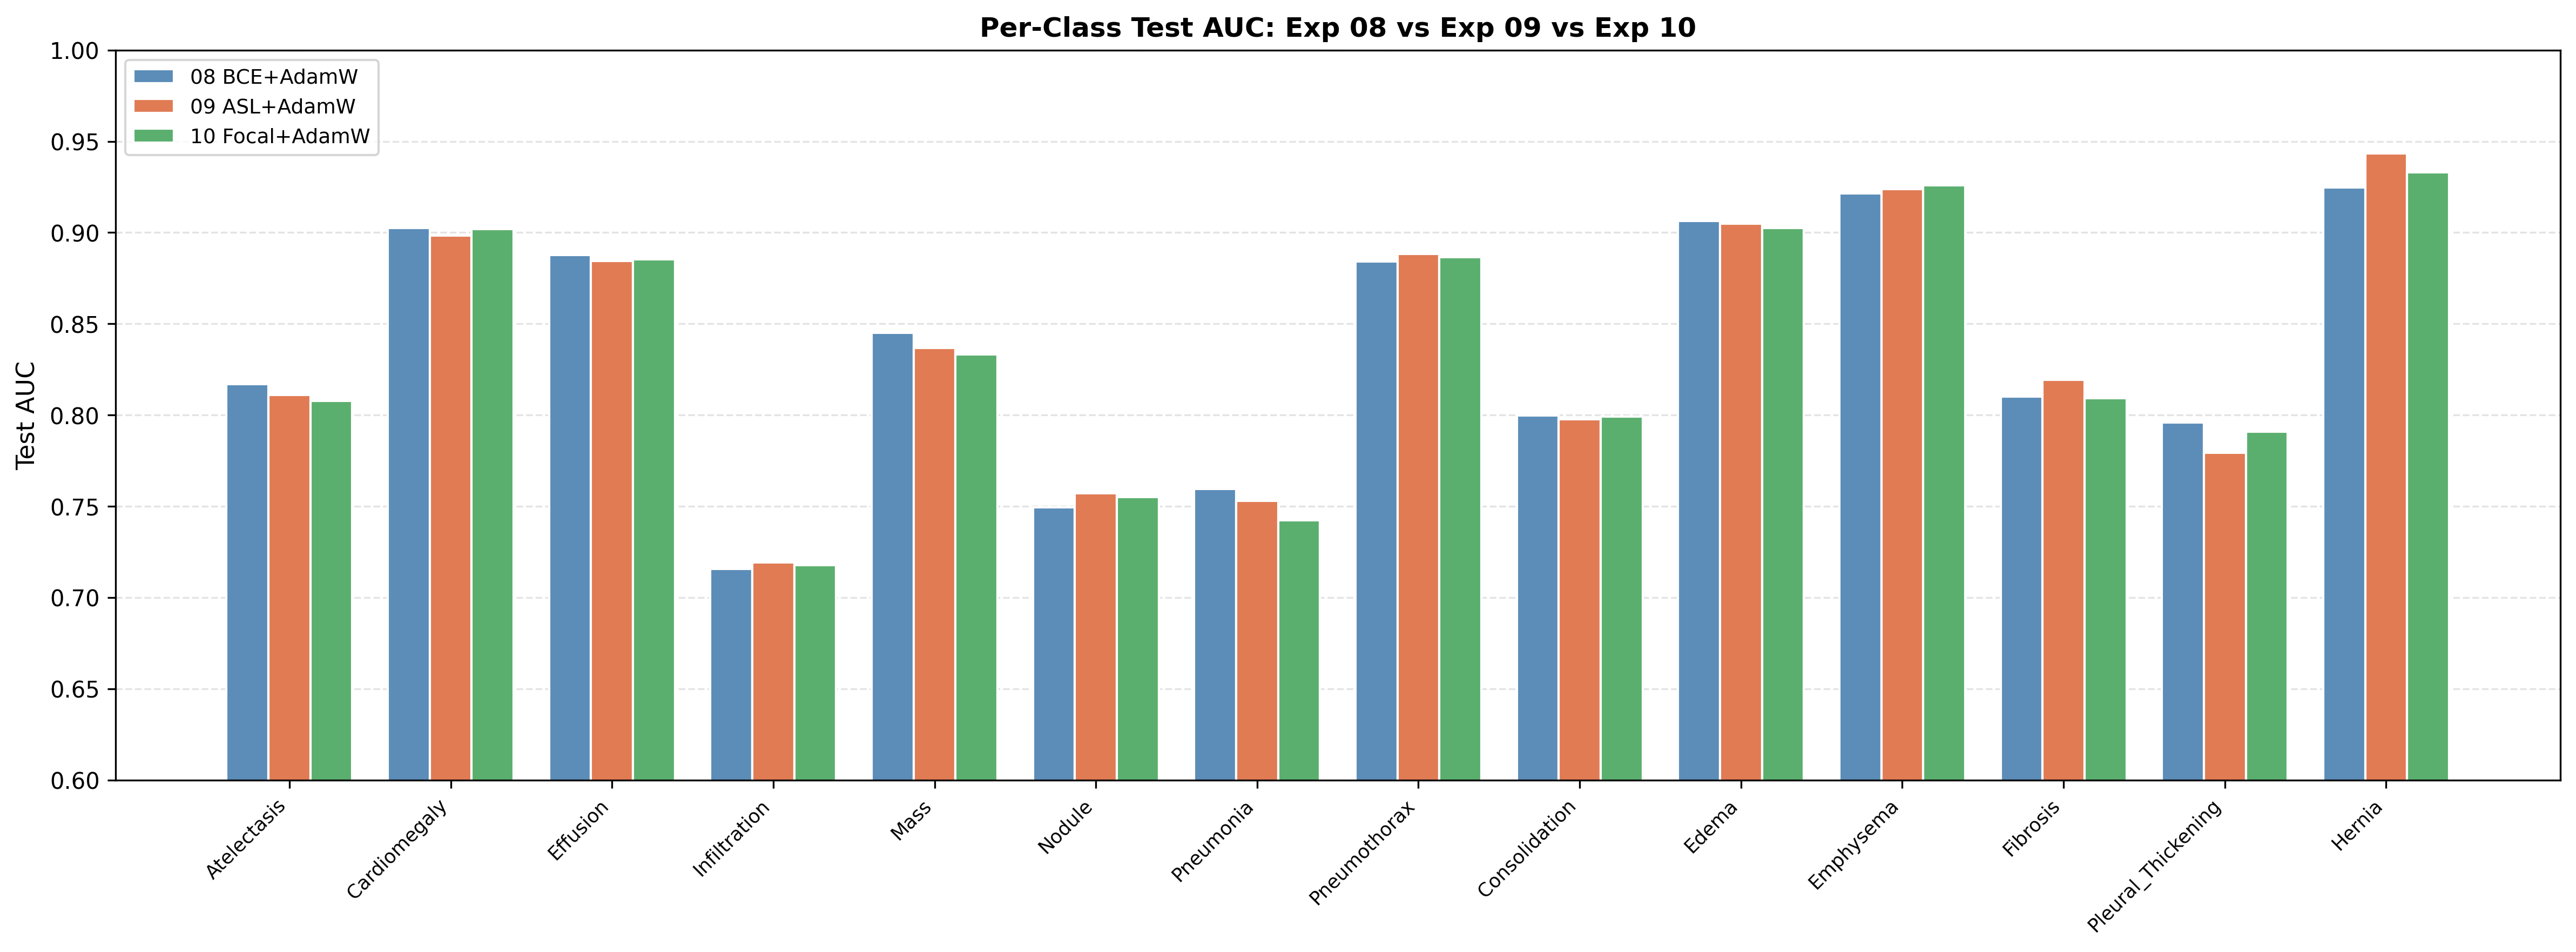
\includegraphics[width=\linewidth]{figures/per_class_auc_best_models.png}
  \caption{Per-class Test AUC for Experiments~08 (BCE + AdamW), 09 (ASL + AdamW),
    and 10 (Focal + AdamW). Classes are ordered as in the NIH ChestX-ray14 label set.
    Hernia, Emphysema, and Edema are the strongest classes; Infiltration,
    Pneumonia, and Nodule remain the most challenging.}
  \label{fig:perclass}
\end{figure*}

\subsection{Grad-CAM Qualitative Analysis}

Grad-CAM~\cite{selvaraju2017gradcam} visualizations were generated for selected positive test examples to qualitatively inspect the image regions contributing to model predictions.
Figure~\ref{fig:gradcam_hernia} shows overlays for a positive Hernia test image.

\textbf{Grad-CAM visualizations provide qualitative insight into model behavior, but they should not be interpreted as definitive localization evidence.}
The predicted probabilities for this example differ substantially between the two models (Exp~08: $p = 0.04$; Exp~09: $p = 0.33$), reflecting the recall-oriented behavior of ASL.

\begin{figure}[H]
  \centering
  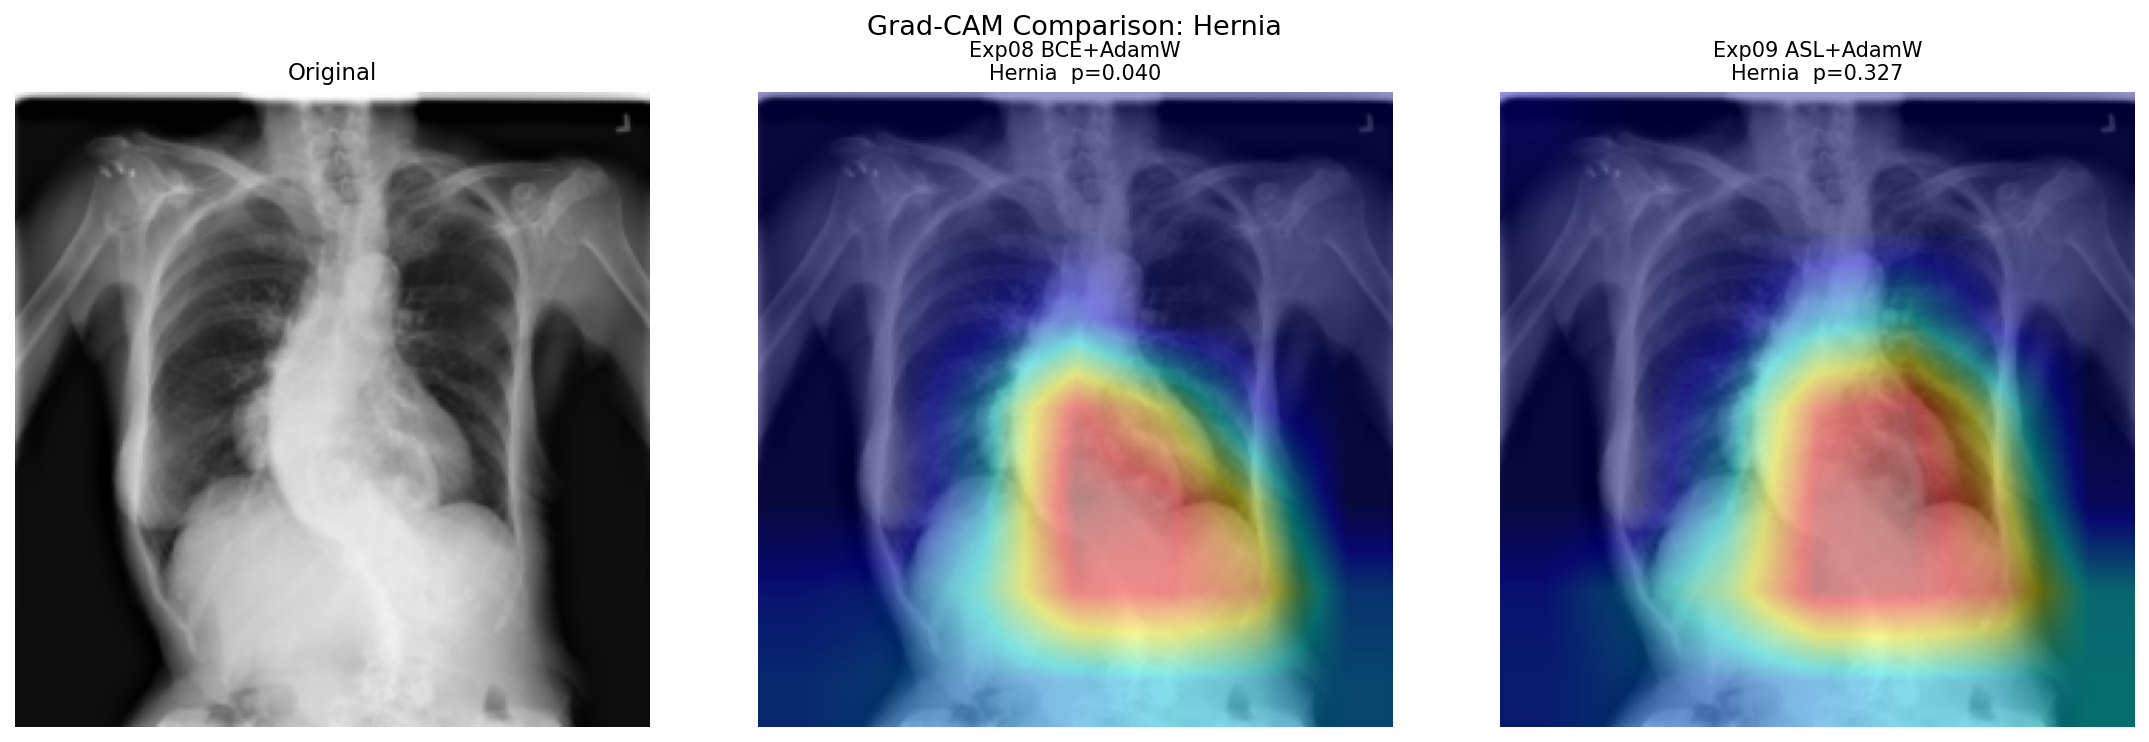
\includegraphics[width=\linewidth]{figures/hernia_example_01_comparison.png}
  \caption{Grad-CAM overlays for a positive Hernia test example.
    \textit{Left}: original image.
    \textit{Center}: Experiment~08 heatmap (predicted probability 0.04).
    \textit{Right}: Experiment~09 heatmap (predicted probability 0.33).
    Experiment~09 (ASL) activates a broader and more prominent region.
    These are qualitative observations only.}
  \label{fig:gradcam_hernia}
\end{figure}

Figure~\ref{fig:gradcam_mass} shows the Experiment~09 Grad-CAM overlay for a positive Mass test example.

\begin{figure}[H]
  \centering
  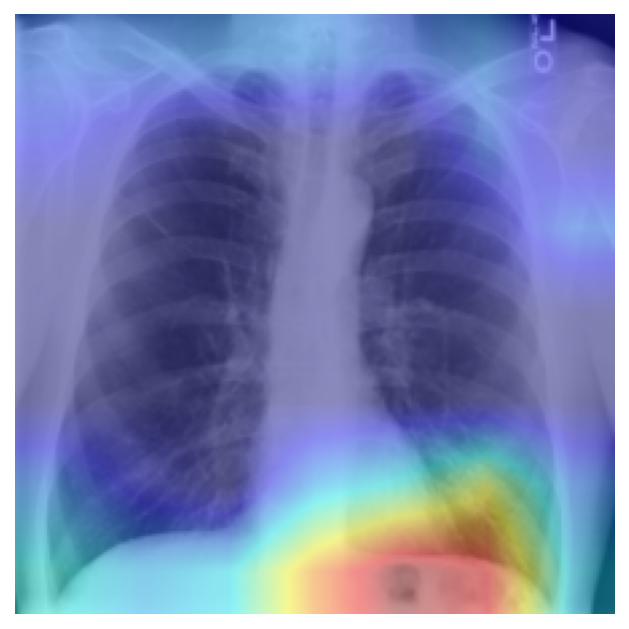
\includegraphics[width=0.75\linewidth]{figures/mass_example_01_exp09_overlay.png}
  \caption{Grad-CAM overlay for a positive Mass test example from Experiment~09.
    The model attends to the central lung region.
    Qualitative observation only; not to be interpreted as localization.}
  \label{fig:gradcam_mass}
\end{figure}

\subsection{Ablation: CBAM Placement}

Three CBAM placement variants were evaluated on DenseNet121 with CLAHE and BCE (Experiments~03a, 03b, 03c):
block4 achieved Mean Test AUC~0.8323, block34 achieved 0.8359, and block1234 achieved 0.8343.
CBAM block34 was selected as the best placement and fixed for all subsequent experiments.

\subsection{Negative Results}

Focal Loss with $\gamma{=}2.0$ (Experiment~10, AUC~0.8351) did not improve over BCE (0.8371) or ASL (0.8370).
FAAR (Frequency-Aware Attention Refinement, Experiments~05 and 05b) was also evaluated as an additional attention mechanism; it did not improve Mean Test AUC (approximately 0.831) over the non-FAAR ASL baseline (0.834) and was not included in final model candidates.
